\documentclass{article}[12pt]

%---------Packages----------
\usepackage{amsmath}
\usepackage{amsfonts}
\usepackage{amssymb}
\usepackage{amsthm}
\usepackage{enumerate}
\usepackage{graphicx}
\usepackage{fancyhdr}
\usepackage{tikz}
\usepackage{dcolumn}
\usepackage{pgfplots}
\pgfplotsset{compat=newest}

%---------Environments----------
\theoremstyle{definition}
\newtheorem{problem}{Problem} %Allows tex to count up the problems for me
\newtheorem*{bonus}{Bonus Problem} %In cases there are ever any bonus problems

\newcommand{\bprob}{\begin{problem}} %Allows me to be lazy and type \bprob instead of \begin{problem}
\newcommand{\eprob}{\end{problem}}

\numberwithin{equation}{problem} %Numbers equations within the problem instead of for the entire document

\newcolumntype{d}[1]{D{.}{.}{#1}}
\newcommand\mc[1]{\multicolumn{1}{c}{#1}} % handy shortcut macro

%----------PageStyleStuff----------
\textwidth=6.5in
\textheight=8.0in
\topmargin=0in
\oddsidemargin=0in
\evensidemargin=0in
% I like to put a header and footer on each page with my name and the assignment in the header and the page number in the footer
\pagestyle{fancy}
\lhead{Parallel Algorithms, Assignment $1$}
\chead{}
\rhead{Ziji Zhang, Jinku Cui}
\lfoot{}
\cfoot{\thepage}
\rfoot{}

\begin{document}
\bprob
Run the code as is to find ranges of \textbf{CAPACITY} and \textbf{NUMITEMS} that require around 10 seconds to run.

\begin{table}[htbp]
\centering
\begin{tabular}{|c|c|c|c|c|}
\hline
\multicolumn{1}{|c|}{Capacity} & \multicolumn{1}{c|}{Items} & \multicolumn{1}{c|}{\begin{tabular}[c]{@{}c@{}}Memory inefficient\\ (value \& solution)\end{tabular}} & \multicolumn{1}{c|}{\begin{tabular}[c]{@{}c@{}}Memory efficient\\ (value only)\end{tabular}} & \multicolumn{1}{c|}{\begin{tabular}[c]{@{}c@{}}Memory efficient\\ (value \& solution)\end{tabular}} \\ \hline
50,000 & 5,000 & 15.8426 & 5.81777 & 13.6626 \\ \hline
25,000 & 10,000 & 12.6301 & 5.68191 & 13.2752 \\ \hline
100,000 & 2,500 & 12.6167 & 5.97705 & 14.1457 \\ \hline
\end{tabular}
\caption{\label{tab:table-name}Some sets of capacity and number of items that run at around 10 seconds}
\end{table}
% record some of the running times and draw some conclusions from what you observe
Observation: Here, the products of capacity and item are all close to 250,000,000.\\
\indent Conclusion: due to the runtime complexity of dynamic programming version of knapsack problem $\mathcal{O}(\log{nW})$, we can see that the running time is positively proportional to the number of items and the capacity of the knapsack.
\eprob

\bprob
Read the code and see if there are any cache locality optimizations that could improve performance.\\
\indent As Figure 1 and 2 show, in the memory inefficient part of the code, the way of storing the data doesn't match the way of accessing the data. To optimize this, either we change the way of indexing, or we change the way we access the table. Once they are in the same style (both in column major or both in row major), we achieve the spatial locality of cache.\\
\begin{figure}[h]
  \centering
  \begin{minipage}[b]{0.45\textwidth}
    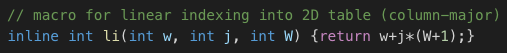
\includegraphics[width=\textwidth]{column_major_declaration.png}
    \caption{Index the data by column major}
  \end{minipage}
  \hfill
  \begin{minipage}[b]{0.45\textwidth}
    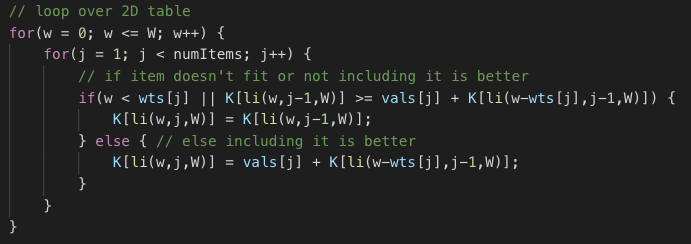
\includegraphics[width=\textwidth]{accessing_row_major.png}
    \caption{Build up table by row major}
  \end{minipage}
\end{figure}

\begin{table}[htbp]
\centering
\begin{tabular}{|r|r|l|l|l|}
\hline
\multicolumn{1}{|c|}{Capacity} & \multicolumn{1}{c|}{Items} & \multicolumn{1}{c|}{\begin{tabular}[c]{@{}c@{}}Memory inefficient\\ (value \& solution)\end{tabular}} & \multicolumn{1}{c|}{\begin{tabular}[c]{@{}c@{}}Memory efficient\\ (value only)\end{tabular}} & \multicolumn{1}{c|}{\begin{tabular}[c]{@{}c@{}}Memory efficient\\ (value \& solution)\end{tabular}} \\ \hline
1000 & 1000 & 0.0260408 & 0.0168568 & 0.384746 \\ \hline
5000 & 1000 & 0.175559 & 0.109112 & 0.244531 \\ \hline
5000 & 5000 & 1.28282 & 0.540613 & 1.20950 \\ \hline
10000 & 1000 & 0.39598 & 0.226099 & 0.516556 \\ \hline
10000 & 10000 & 5.555875 & 2.22395 & 5.07604 \\ \hline
20000 & 2000 & 2.24177 & 0.921218 & 2.13556 \\ \hline
50000 & 5000 & 15.8426 & 5.81777 & 13.6626 \\ \hline
100000 & 10000 & 66.9352 & 23.3454 & 55.9303 \\ \hline
\end{tabular}
\caption{\label{tab:original}Running time of original sequential code}
\end{table}

\begin{table}[htbp]
\centering
\begin{tabular}{|r|r|l|l|l|}
\hline
\multicolumn{1}{|c|}{Capacity} & \multicolumn{1}{c|}{Items} & \multicolumn{1}{c|}{\begin{tabular}[c]{@{}c@{}}Memory inefficient\\ (value \& solution)\end{tabular}} & \multicolumn{1}{c|}{\begin{tabular}[c]{@{}c@{}}Memory efficient\\ (value only)\end{tabular}} & \multicolumn{1}{c|}{\begin{tabular}[c]{@{}c@{}}Memory efficient\\ (value \& solution)\end{tabular}} \\ \hline
1000 & 1000 & 0.0212187 & 0.0168568 & 0.384746 \\ \hline
5000 & 1000 & 0.133945 & 0.109112 & 0.244531 \\ \hline
5000 & 5000 & 0.668835 & 0.540613 & 1.20950 \\ \hline
10000 & 1000 & 0.273084 & 0.226099 & 0.516556 \\ \hline
10000 & 10000 & 2.73563 & 2.22395 & 5.07604 \\ \hline
20000 & 2000 & 1.12666 & 0.921218 & 2.13556 \\ \hline
50000 & 5000 & 7.13521 & 5.81777 & 13.6626 \\ \hline
100000 & 10000 & 29.0102 & 23.3454 & 55.9303 \\ \hline
\end{tabular}
\caption{\label{tab:cacheLocality}Running time with cache locality}
\end{table}

\indent Table 2 and 3 are the records for the original sequential code before and after we achieve the spatial locality of cache for memory inefficient part (so only the results under Memory inefficient column change). From the results, we can see that for small capacity and number of items, the improvement in time is about $20\%$; when the capacity and number become large, the improvement in time is increased above $50\%$ which is decent.
\eprob

\bprob
Use \textbf{OpenMP} to parallelize each of the 3 algorithms in a new file called knapsack\_parallel.cpp

% memory inefficient (value & solution), memory efficient (value only), memory efficient (value & solution)
% measure your parallel performance and record strong scaling results
% draw some conclusions from what you observe

\begin{table}[hb]
\centering
\begin{tabular}{|r|r|l|l|l|}
\hline
Capacity & Items & \multicolumn{1}{c|}{\begin{tabular}[c]{@{}c@{}}Memory inefficient\\ (value \& solution)\end{tabular}} & \multicolumn{1}{c|}{\begin{tabular}[c]{@{}c@{}}Memory efficient\\ (value only)\end{tabular}} & \multicolumn{1}{c|}{\begin{tabular}[c]{@{}c@{}}Memory efficient\\ (value \& solution)\end{tabular}} \\ \hline
1000 & 1000 & 0.030061 & 0.0168941 & 0.131404 \\ \hline
5000 & 1000 & 0.0436337 & 0.02075 & 0.13755 \\ \hline
5000 & 5000 & 0.181331 & 0.0728484 & 0.788706 \\ \hline
10000 & 1000 & 0.0679167 & 0.0229069 & 0.151138 \\ \hline
10000 & 10000 & 0.50116 & 0.20791 & 1.88364 \\ \hline
20000 & 2000 & 0.18389 & 0.0587676 & 0.324667 \\ \hline
50000 & 5000 & 1.0174 & 0.307317 & 1.32777 \\ \hline
100000 & 10000 & 8.83435 & 1.10914 & 4.01752 \\ \hline
\end{tabular}
\caption{\label{tab:parallelized}Parallelized code with spatial locality on 32 cores}
\end{table}

\begin{itemize}
    \item \textbf{Memory inefficient (value \& solution) }
    This algorithm involves $2$ methods: \textit{build\_table}() and \textit{backtrack}().
    
    The \textit{build\_table}() method contains $2$ \textit{for} loops. The first \textit{for} loop initializes first column, and we add the OpenMP parallel for directive before it. The second one is a nested \textit{for} loop. We interchange the outter and inner \textit{for} loop and then add OpenMP directive exactly before the inner loop.
    
    We do not change the \textit{backtrack}() method. Even though it contains a \textit{for} loop, there exists write-after-read dependency. The for loop cannot be parallelized.
    
    \item \textbf{Memory efficient (value only)}
    This algorithm is related with only $1$ method: \textit{compute\_table}(). 
    
    The structure of that method is quite similar with the \textit{build\_table}() method, and it includes a simple \textit{for} loop and a nested \textit{for} loop. Similarly, we wrap the single \textit{for} loop with OpenMP directive, and we add pragma to the inner \textit{for} loop of the nested loop statements.
    
    \item \textbf{Memory efficient (value \& solution)}
    This algorithm contains \textit{backtrack\_implicit}() and \textit{convert\_path\_to\_used}() methods.
    
    The \textit{backtrack\_implicit}() is recursive and therefore we do not parallelize it directly. However, it depends on a subroutine called \textit{findk}() method. We parallelize the first simple \textit{for} loop and the inner \textit{for} loop of the second nested \textit{for} loop statements.
    
    The \textit{for} loop in \textit{convert\_path\_to\_used}() method needs to modify a variable, and we need to put the whole block of the \textit{for} loop in a critical region if we want to parallelize the \textit{for} loop. It is meaningless to create the paradox.
    
\end{itemize}

\indent We run the \textit{knapsack\_parallel} on a node with $32$ cores, and the running times for different configuration are recorded in Table ~\ref{tab:parallelized}. With comparing with the data in Table \ref{tab:cacheLocality}, the speedup seems trivial when the size of the problem is relative small, e.g. $capacity=1000, items=1000$. The running time for the first two algorithm is almost the same. The third algorithm is as three times fast as the original version. When we test these three algorithm with parameter $capacity=10000, items=10000$, the first algorithm is as $5$ times fast as before, the second algorithm is as $11$ times fast as before, and the third algorithm is as $3$ times fast as the initial version. Figure \ref{fig:runningTimePlot} illustrates the trend of execution time on different configurations.

\begin{figure}[ht]  
\begin{center}  

\begin{tikzpicture}[scale = 1]
\begin{axis}[
        legend cell align = left,
        legend pos = north west,
        width=\textwidth,
        height=0.6\textwidth,
        title = Running time of the original and modified algorithms,
        xlabel = Product of Capacity \& Items,
        ylabel = Running time (seconds),
        legend entries = {Mem inef (val \& sol),
        Mem eff (val only),
        Mem eff (val \& sol),
        Cache localized mem inef (val \& sol),
        Parallelized mem inef (val \& sol),
        Parallelized mem eff (val only),
        Parallelized mem eff (val \& sol)}
        ]
\addplot[blue, thin, mark=star] table[x = Probsize, y = Meminefsol] {time.txt};
\addplot[blue, thin, mark=square*] table[x = Probsize, y = Memeffval] {time.txt};
\addplot[blue, thin, mark=diamond*] table[x = Probsize, y = Memeffsol] {time.txt};

\addplot[green, thin, mark=star, dash dot] table[x = Probsize, y = Cache] {time.txt};

\addplot[red, thin, mark=star, dashed] table[x = Probsize, y = Pmis] {time.txt};
\addplot[red, thin, mark=square*, dashed] table[x = Probsize, y = Pmev] {time.txt};
\addplot[red, thin, mark=diamond*, dashed] table[x = Probsize, y = Pmes] {time.txt};

\end{axis}
\end{tikzpicture}  

\label{fig:runningTimePlot}  
\end{center}

\caption{Execution time of the sequential and parallel algorithms, as well as the one with cache locality. The $x$ axis represents the product of capacity value and item numbers. The $y$ axis denote the running time in seconds. Blue solid lines represents sequential algorithms, and the red dashed lines indicate parallelized algorithms. The green dash dot line stands for running time of the memory inefficient algorithm with cache locality.}
\end{figure}  


\eprob

\end{document}